%!TEX root = main.tex
\section{Missing Figures}
\label{sec:fig}

\begin{figure}[H]
\centering
\begin{tikzpicture}
 \filldraw[fill=green!20!white]
 (0,4)--(10,4)--(10,5)--(0,5)--cycle;
 \foreach \x in {0,3,8}
 {
 \filldraw[fill=blue!20!white]
 (\x+0,2)--(\x+2,2)--(\x+2,3)--(\x+0,3)--cycle;
 \draw (\x+1,3)--(5,4);
 \filldraw[fill=red!20!white]
 (\x+0,0)--(\x+2,0)--(\x+2,1)--(\x+0,1)--cycle;
 \draw (\x+1,1)--(\x+1,2);
 \draw(\x+0.33,1)--(\x+1,2);
 \draw(\x+1.66,1)--(\x+1,2);
 %\draw(\x+1.4,1)--(\x+1,2);
 %\draw(\x+1.8,1)--(\x+1,2);
 \draw(\x+0.66,0)--(\x+0.66,1);
 \draw(\x+1.33,0)--(\x+1.33,1);
% \draw (\x+1.2,0)--(\x+1.2,1);
 %\draw(\x+1.6,0)--(\x+1.6,1);
 \node at(\x+1,2.5){$T_2$ rounds};
 \node at(\x+0.33, 0.5){$\GdT$};
 %\node at(\x+0.6, 0.5){$\cdot$};
 \node at(\x+1.0, 0.5){$\cdots$};
 %\node at(\x+1.4, 0.5){$\cdot$};
 \node at(\x+1.66, 0.5){$\GdT$};
 %\node at(\x+1,0.5){$T_1 \cdot \GdT$};
 \draw [decorate,decoration={brace,amplitude=10pt},xshift=0pt,yshift=0pt] (\x+2,-0.2) -- (\x+0,-0.2) node [black,midway,yshift=-0.6cm] {$T_1$ paths};
 }
  \node at(5,4.5){all remaining rounds};
  \node at (6,0.5){$\cdots$};
  \node at (7,0.5){$\cdots$};
  \node at (6,2.5){$\cdots$};
  \node at (7,2.5){$\cdots$};
  \node at(-1,0.5){\textbf{Level 1}};
  \node at(-1,2.5){\textbf{Level 2}};
  \node at(-1,4.5){\textbf{Level 3}};
  \draw[->] (11,0)--(11,5);
  \node at(11.5,2.5)[ rotate=90]{Time};

  \draw [decorate,decoration={brace,amplitude=10pt,aspect=0.33},xshift=0pt,yshift=0pt] (10,1.8) -- (0,1.8) node [black,pos=0.33,xshift = 0cm,yshift=-0.6cm] {$\NG$ groups};

\end{tikzpicture}
\caption{Info-graph for the three-level policy. Each red box in level 1 corresponds to $T_1$ full-disclosure paths of length $\GdT$ each.}
\label{fig:3level}
\end{figure}


\begin{figure}[H]
\centering
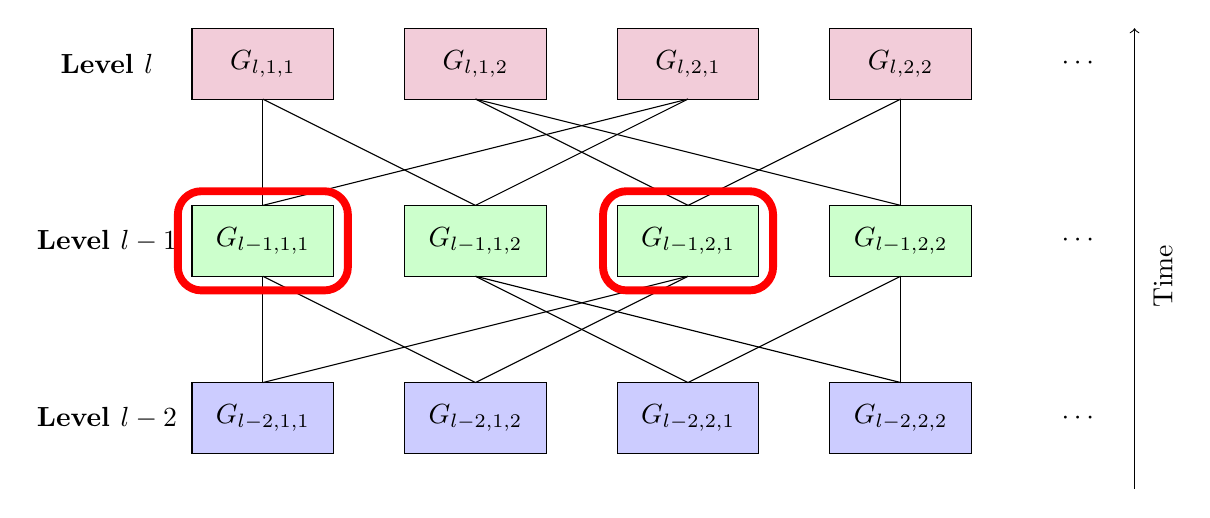
\begin{tikzpicture} [scale = 0.9]
 \foreach \x in {0,3,6,9}
 {
 \filldraw[fill=purple!20!white]
 (\x+0,7.5)--(\x+2,7.5)--(\x+2,8.5)--(\x+0,8.5)--cycle;
 \filldraw[fill=green!20!white]
 (\x+0,5)--(\x+2,5)--(\x+2,6)--(\x+0,6)--cycle;
 \filldraw[fill=blue!20!white]
 (\x+0,2.5)--(\x+2,2.5)--(\x+2,3.5)--(\x+0,3.5)--cycle;
 }
\foreach \y in {2.5,5,7.5}
{
  \node at (12.5,\y+0.5){$\cdots$};
}


\foreach \y in {3.5,6}
{
  \draw (1,\y) -- (1,\y+1.5);
  \draw (1,\y) -- (7,\y+1.5);

  \draw (4,\y) -- (1,\y+1.5);
  \draw (4,\y) -- (7,\y+1.5);


  \draw (7,\y) -- (4,\y+1.5);
  \draw (7,\y) -- (10,\y+1.5);


  \draw (10,\y) -- (4,\y+1.5);
  \draw (10,\y) -- (10,\y+1.5);
}

\foreach \u in {1,2}
{
	\foreach \v in {1,2}
	{
	\pgfmathsetmacro{\x}{((\u-1)*2+(\v-1))*3};
	\pgfmathsetmacro{\xa}{((\u-1))*3};
	\pgfmathsetmacro{\xb}{(2+(\u-1))*3};
   \node at(\x+1,8){$G_{l,\u,\v}$};
   \node at(\x+1,5.5){$G_{l-1,\u,\v}$};
   \node at(\x+1,3){$G_{l-2,\u,\v}$};
	}
}


  \node at(-1.2,3){\textbf{Level $l-2$}};
  \node at(-1.2,5.5){\textbf{Level $l-1$}};
  \node at(-1.2,8){\textbf{Level $l$}};
  \draw[->] (13.3,2)--(13.3,8.5);
  \node at(13.7,5)[ rotate=90]{Time};

 \draw [rounded corners=3mm, line width=1mm, red](-0.2,4.8)--(2.2,4.8)--(2.2,6.2)--(-0.2,6.2)--cycle;
  \draw [rounded corners=3mm, line width=1mm, red](5.8,4.8)--(8.2,4.8)--(8.2,6.2)--(5.8,6.2)--cycle;
\end{tikzpicture}
\caption{Interlacing connections between levels for the $L$-level policy.}
\label{fig:llevel-connecting}
\end{figure}


%%% Local Variables:
%%% mode: latex
%%% TeX-master: "main"
%%% End:
